\section{Anwendungen}
\subsection{Dieelektrische Berechnung von Hochspannungsgeräten}
\begin{itemize}
	\item Das elektrische Feld einer geometrischen Anordnung hängt von den Abständen zwischen den Elektroden und den geerdeten Flächen ab.
	\item Die Felderhöhung entsteht an scharfen Ecken und Kanten
	\item Abrundung dieser scharfen Stellen verringert das elektrische Feld
	\item Falls eine Abrundung nicht möglich ist, wird eine elektrische Abschirmung eingebaut
\end{itemize}
\subsection{Wirbelströme in Transformatoren}
\begin{itemize}
	\item Das magnetische Streufeld eines Transformators induziert in den Wicklungen Wirbelströme
	\item Diese Wirbelströme sorgen für eine zusätzliche Erwärmung der Bauteile im Trafo
	\item Die Wirbelströme können nur über Simulationen berechnet werden. 
\end{itemize}
\subsection{Elektromagnetische Analyse von Elektrischen Maschinen}
\begin{itemize}
	\item Das magnetische Feld wird durch die Statorwicklung erzeugt
	\item Die Leiter im Rotor werden vom magnetischen Feld durchflossen. Durch die magnetischen Kräfte des Feldes wird das Drehmoment erzeugt. 
	\item Durch Simulationen können die Kennwerte der elektrischen Maschine berechnet werden
\end{itemize}
\subsection{Eigenwertanalyse von Wellenleitern}
\begin{itemize}
	\item Das Design von Wellenleitern basiert auf der Eigenwertanalyse
	\item Eigenwertanalyse: Eigenwert (Wellenausbreitungskonstante), Eigenvektor (Feldverteilung für gegebene Frequenz)
\end{itemize}
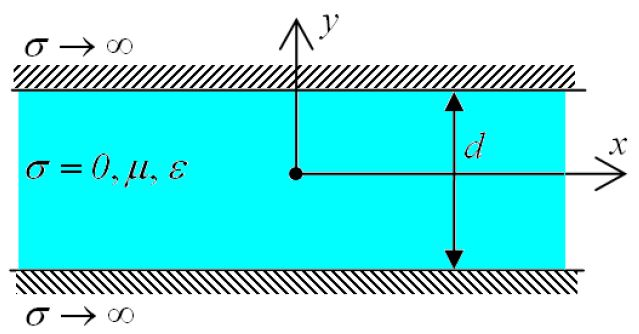
\includegraphics[width=6cm]{images/Wellen.jpg}\\
\begin{tabular}{|p{0.45\textwidth} |p{0.45\textwidth}|}
	\hline
	\textbf{Wellengleichung}\newline
	$\dfrac{d^2E}{dy^2}+(\omega^2-\mu\epsilon-\gamma^2)E_z=0 $&
	\textbf{Lösung der Wellengleichung}\newline
	$E= \underbrace{A\cos(k\cdot y)\cdot \euler^{-j\frac{\gamma}{y}}}_{\text{Even Modes}} + \underbrace{B\sin(k\cdot y)\cdot \euler^{-j\frac{\gamma}{x}}}_{\text{Odd Modes}} $ \\
	\hline
	\textbf{Even Mode}\newline
	$\cos(k \cdot \frac{\pm d}{2}) \rightarrow k=\frac{2n+1}{d} \cdot \pi $\newline
	\tabbild[width=6cm]{images/Even.jpg}
	&
	\textbf{Odd Mode}\newline
	$\sin(k \cdot \frac{\pm k}{2}) \rightarrow k=\frac{2n}{d} \cdot \pi $\newline
	\tabbild[width=6cm]{images/Odd.jpg}\\
	\hline
\end{tabular}
\vspace{0.5cm}\\
\subsubsection{Eigenwertanalyse Homogener Wellenleiter}
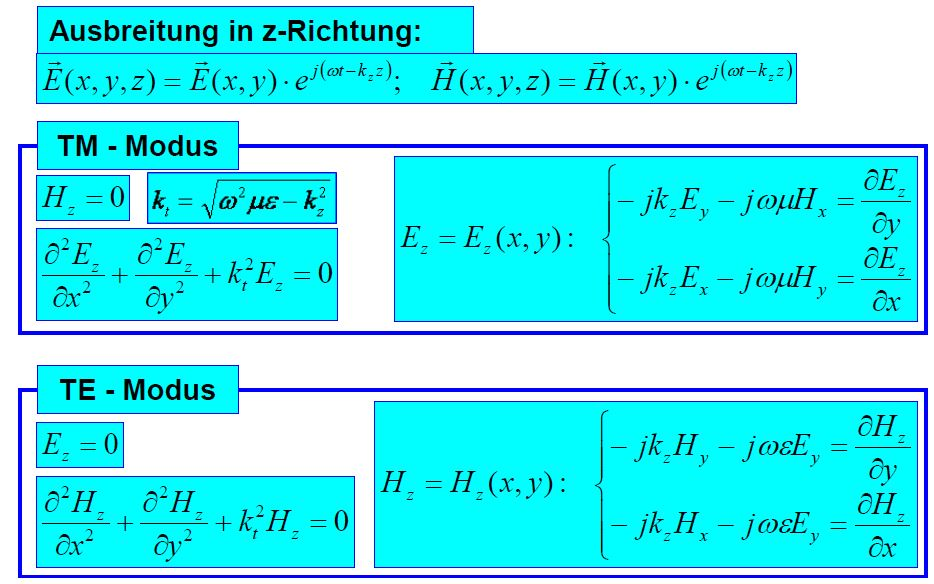
\includegraphics[width=0.8\linewidth]{images/Eigenwertanalyse.jpg}